
\documentclass{exam}

\usepackage{units} 
\usepackage{graphicx}
\usepackage[fleqn]{amsmath}
\usepackage{cancel}
\usepackage{float}
\usepackage{mdwlist}
\usepackage{booktabs}
\usepackage{cancel}
\usepackage{polynom}
\usepackage{caption}
\usepackage{fullpage}
\usepackage{xfrac}
\usepackage{enumerate}

\newcommand{\degree}{\ensuremath{^\circ}} 
\everymath{\displaystyle}

% \begin{figure}[H]
%   \centering
%   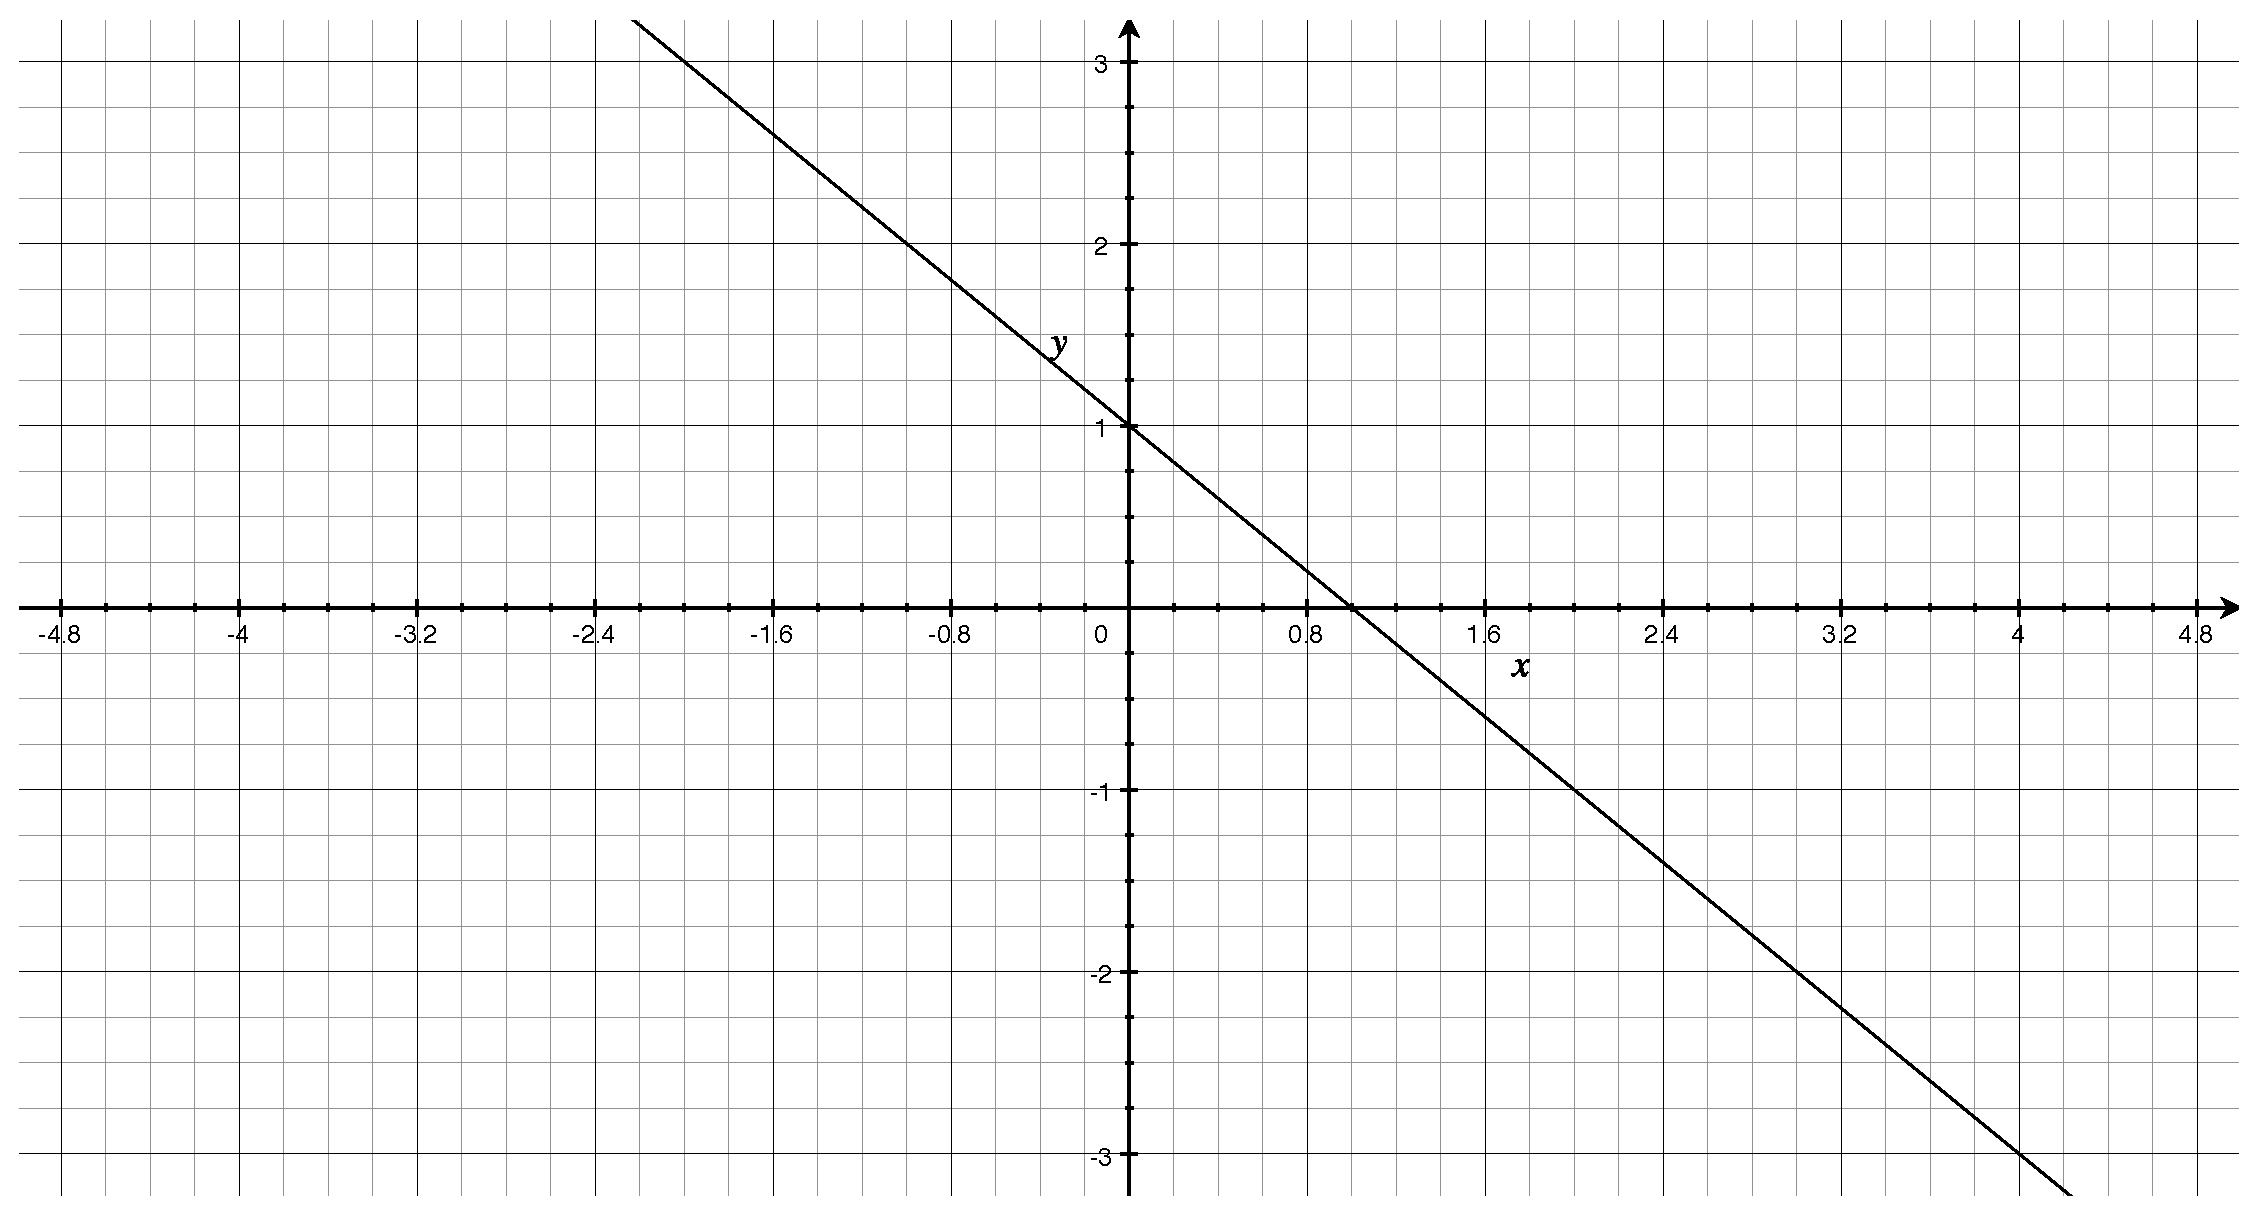
\includegraphics[scale=.3]{problem7.eps}
%   \caption*{Problem 7}
% \end{figure}

% \begin{tabular}{cc}
%   \toprule
%   period & amplitude \\
%   \midrule
%   value one & value two
%   \bottomrule
% \end{tabular}

\printanswers

\ifprintanswers 
  \usepackage{2in1, lscape} 
\fi

\date{May 15, 2013}
\author{}
\title{Math 141 \\ Homework 12}

\begin{document}

\maketitle


\section{Homework}

\begin{itemize*}
  \item Read Section 4.1 
  \item Section 4.1: 
\end{itemize*}

\section{Extra Credit}
  TO DO 

\ifprintanswers
  \pagebreak

  \begin{description}
    \item[1] TO DO

  \end{description}

  \pagebreak

  \section{Section 4.1}

  \begin{description}

    \item[5] TO DO

  \end{description}

\else
  \vspace{6 cm}
  \begin{quote}
    \begin{em}
      TO DO
    \end{em}
  \end{quote}

  \hspace{1 cm} --author here


\fi

\end{document}

